\documentclass[11pt,a4paper]{article}

\usepackage[english]{babel}
\usepackage[utf8]{inputenc}
\usepackage[T1]{fontenc}
\usepackage{geometry}
\usepackage{graphicx}
\usepackage{booktabs}
\usepackage{array}
\usepackage{float}
\usepackage{hyperref}
\usepackage{xcolor}
\usepackage{amsmath}
\usepackage{caption}
\usepackage{subcaption}

\geometry{margin=2.5cm}
\hypersetup{
    colorlinks=true,
    linkcolor=blue!50!black,
    citecolor=blue!50!black,
    urlcolor=blue!50!black
}

\title{\textbf{Blood cell classification using convolutional networks and transfer learning}}
\author{Christian Borasino \and Rody Vilchez}
\date{\today}

\begin{document}

\maketitle

\begin{abstract}
This report summarizes the work developed in the project notebooks to classify blood cell images into four classes: eosinophils, lymphocytes, monocytes, and neutrophils. An exploratory analysis of the dataset was performed, convolutional architectures trained from scratch based on LeNet-5 and a reduced VGG-11 were trained, the effect of Batch Normalization was studied, and three transfer learning strategies with ResNet18 pretrained on ImageNet were compared. The best overall result was obtained by ResNet18 with partial fine-tuning, with a test accuracy of 86.45\%, followed by full fine-tuning with 86.09\% and by the reduced VGG-11 with Batch Normalization with 81.22\%. The critical analysis shows that transfer learning improves performance, but also reveals methodological risks: possible data leakage between partitions, overfitting in some models, and repeated use of the TEST set as a selection criterion.
\end{abstract}

\section{Introduction}

Automatic blood cell classification from microscopic images is a relevant task for supporting hematological analysis processes. Although convolutional networks have shown strong performance in computer vision, their effectiveness depends heavily on the size of the dataset, the stability of training, and the model's ability to learn fine morphological patterns.

The objective of the project was to compare models trained from scratch against models using transfer learning. To this end, five main notebooks were developed: \texttt{01\_eda.ipynb}, dedicated to exploratory analysis; \texttt{02\_lenet.ipynb}, with LeNet-5 experiments; \texttt{02\_vgg.ipynb}, with a reduced VGG-11; the comparative notebook \texttt{02\_comparision.ipynb}, with the study of Batch Normalization, learning rates, and feature maps; and \texttt{03\_transfer.ipynb}, with transfer learning using ResNet18.

\section{Data and exploratory analysis}

The classification dataset is organized in a format compatible with \texttt{ImageFolder}, with \texttt{TRAIN}, \texttt{TEST}, and \texttt{TEST\_SIMPLE} partitions. Four balanced training classes were used: \texttt{EOSINOPHIL}, \texttt{LYMPHOCYTE}, \texttt{MONOCYTE}, and \texttt{NEUTROPHIL}. Table~\ref{tab:distribucion} summarizes the image distribution.

\begin{table}[H]
\centering
\caption{Image distribution by partition and class.}
\label{tab:distribucion}
\begin{tabular}{lrrrrr}
\toprule
Partition & EOSINOPHIL & LYMPHOCYTE & MONOCYTE & NEUTROPHIL & Total \\
\midrule
TRAIN & 2497 & 2483 & 2478 & 2499 & 9957 \\
TEST & 623 & 620 & 620 & 624 & 2487 \\
TEST\_SIMPLE & 13 & 6 & 4 & 48 & 71 \\
\midrule
Total & 3133 & 3109 & 3102 & 3171 & 12515 \\
\bottomrule
\end{tabular}
\end{table}

The EDA found that the most frequent dimension was $320 \times 240$ pixels across the 12515 classification images. The training balance was adequate, with a maximum/minimum ratio of approximately 1.01 across classes. The original annotated set was also reviewed; it contains \texttt{labels.csv} with 411 rows and 15 multi-label cases. The Pascal VOC-style XML annotations include 343 annotated images and 3854 objects labeled as RBC. This suggests that the XML annotations do not directly describe the same task as leukocyte-type classification, but rather localized cellular objects within the image.

An important finding was the presence of 2 groups of exact hash duplicates and 48 source identifiers present in more than one partition. This point is methodologically critical because it may produce information leakage between training and testing, inflating the observed performance. Therefore, the results should be interpreted as an internal experimental comparison and not as a definitive estimate of clinical performance.

\section{Methodology}

\subsection{Preprocessing}

For the models trained from scratch, the images were resized to $64 \times 64$ pixels. For ResNet18, a $224 \times 224$ input was used, consistent with ImageNet pretraining. In all experiments, the images were normalized using the ImageNet mean and standard deviation:
\[
\mu = [0.485, 0.456, 0.406], \qquad \sigma = [0.229, 0.224, 0.225].
\]
In transfer learning, moderate augmentations were incorporated during training to reduce overfitting without aggressively altering cellular morphology.

\subsection{Models trained from scratch}

Two model families were evaluated:

\begin{itemize}
    \item \textbf{Adapted LeNet-5}: architecture with two convolutional layers, \texttt{Tanh} activation, \texttt{AvgPool2d}, and three linear layers. A variant with Batch Normalization after each convolution was implemented.
    \item \textbf{Reduced VGG-11}: VGG-11 version with approximately half the channels, convolutional blocks with \texttt{ReLU}, \texttt{MaxPool2d}, a dense classifier, and \texttt{Dropout}. A variant with Batch Normalization was also evaluated.
\end{itemize}

The models were trained with SGD, learning rate 0.01, momentum 0.9, \texttt{weight\_decay} $5 \times 10^{-4}$, batch size 32, and 10 epochs. Runs were logged in TensorBoard and checkpoints were saved in \texttt{models/}.

\subsection{Transfer learning}

The notebook \texttt{03\_transfer.ipynb} compared three strategies with ResNet18 pretrained on ImageNet:

\begin{itemize}
    \item \textbf{Feature extraction}: the backbone was frozen and only the final layer was trained.
    \item \textbf{Partial fine-tuning}: the first residual blocks were frozen, and \texttt{layer3}, \texttt{layer4}, and the final layer were trained.
    \item \textbf{Full fine-tuning}: the entire network was trained with a small learning rate.
\end{itemize}

The three strategies were trained for 8 epochs using \texttt{TRAIN} for training and \texttt{TEST} for evaluation, with a cosine learning rate scheduler.

\section{Results}

\subsection{Models from scratch}

Table~\ref{tab:desde-cero} shows the best test accuracy observed for the models trained from scratch. The most marked difference appears in the reduced VGG-11: without Batch Normalization, the model remained at performance close to random guessing for four classes, whereas with Batch Normalization it reached 81.22\%.

\begin{table}[H]
\centering
\caption{Best test accuracy in models trained from scratch.}
\label{tab:desde-cero}
\begin{tabular}{lcc}
\toprule
Model & Best TEST accuracy & Main observation \\
\midrule
LeNet-5 & 58.22\% & Learns partially, but with limited capacity. \\
LeNet-5 + BN & 43.83\% & Higher training accuracy, worse generalization. \\
Reduced VGG-11 & 25.09\% & Does not converge; remains close to random guessing. \\
Reduced VGG-11 + BN & 81.22\% & Best model from scratch. \\
\bottomrule
\end{tabular}
\end{table}

In LeNet-5 without Batch Normalization, a progressive training improvement was observed up to 75.33\% training accuracy, but test accuracy oscillated and reached its maximum at 58.22\%. In LeNet-5 with Batch Normalization, training accuracy rose to 96.69\%, while testing remained low and fluctuating, with a maximum of 43.83\%. This reveals overfitting and suggests that Batch Normalization was not sufficient to improve generalization in such a narrow network with \texttt{Tanh} activations.

\begin{figure}[H]
\centering
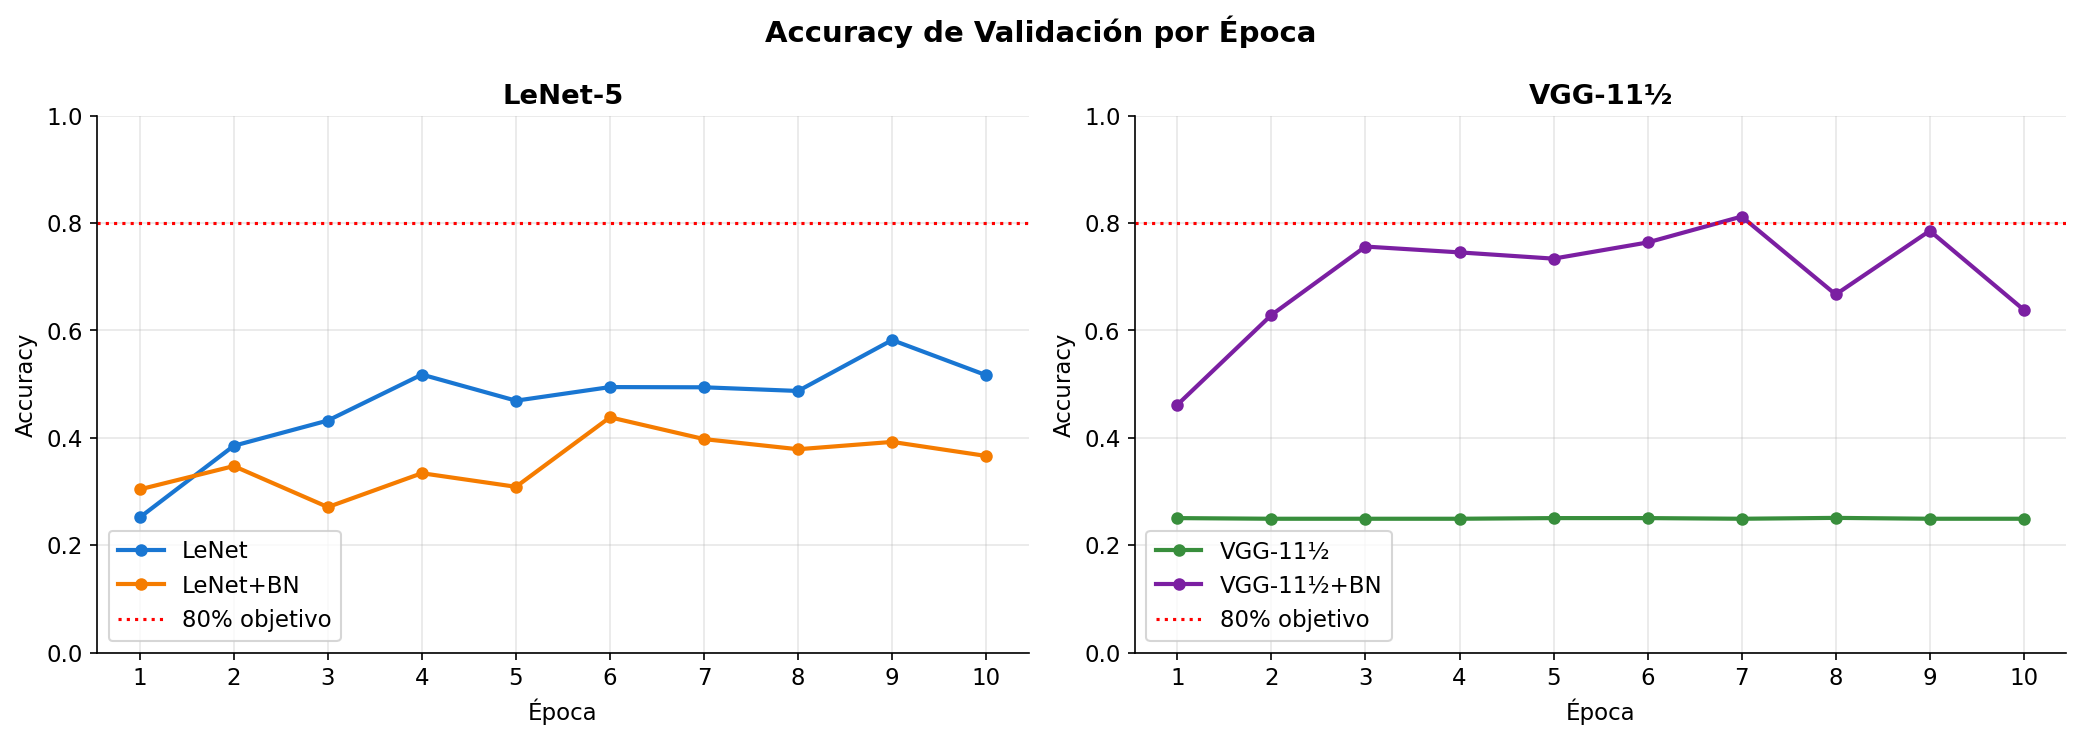
\includegraphics[width=0.92\textwidth]{results/accuracy_curves.png}
\caption{Validation/test accuracy curves for models with and without Batch Normalization.}
\label{fig:accuracy}
\end{figure}

\begin{figure}[H]
\centering
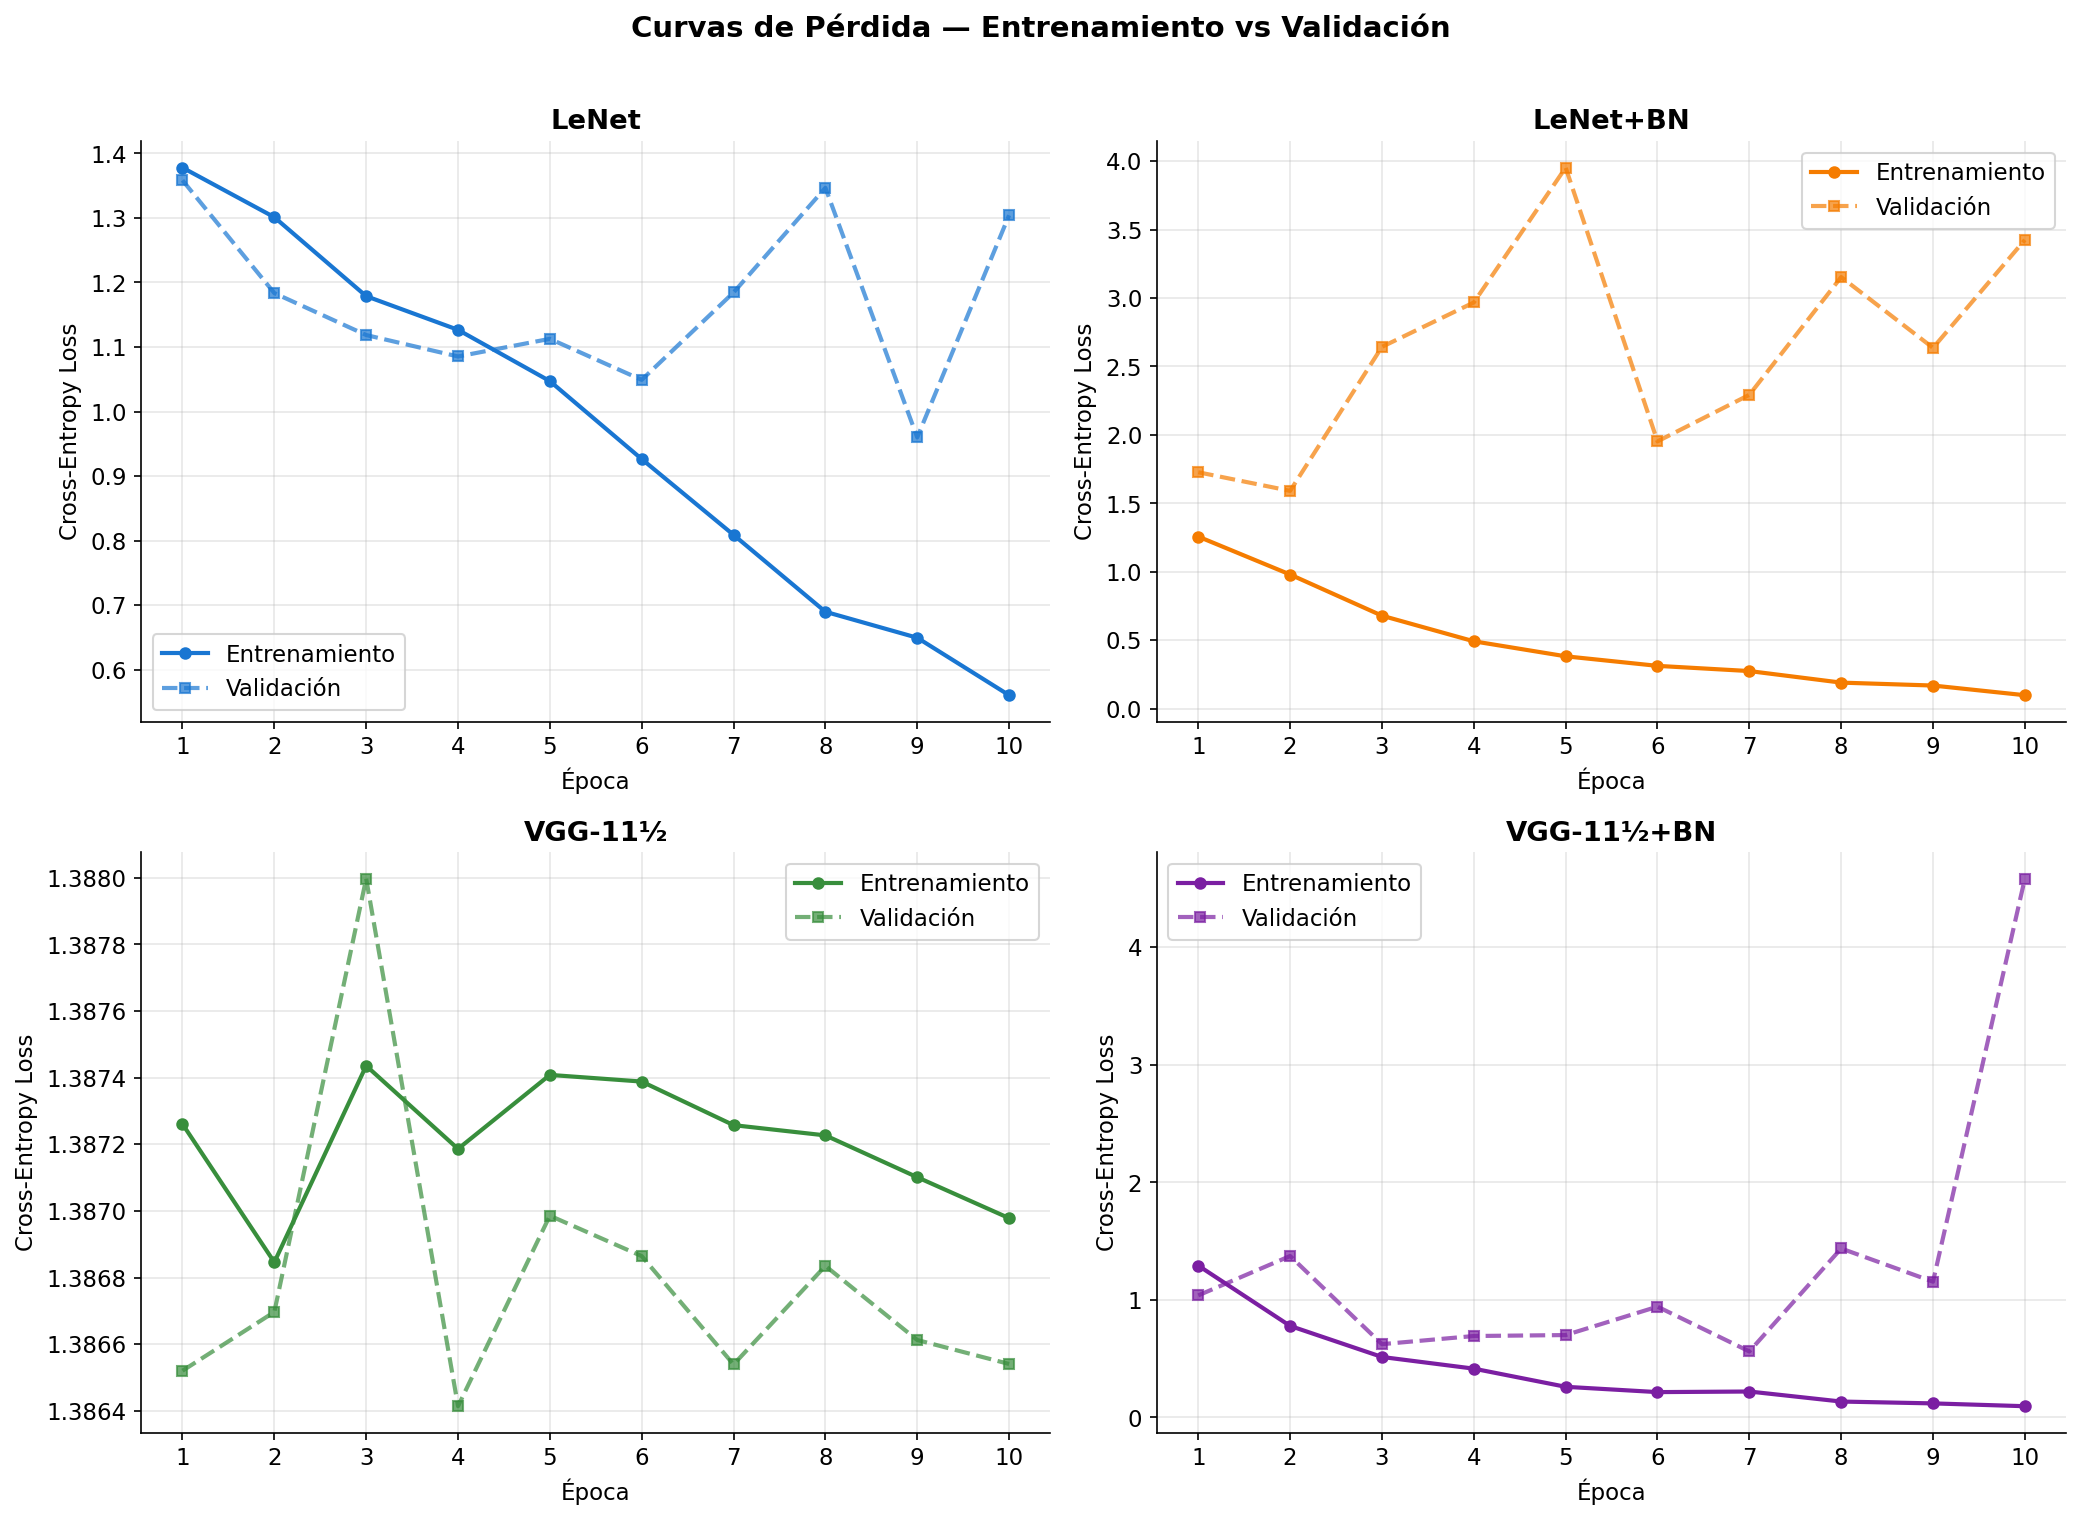
\includegraphics[width=0.92\textwidth]{results/loss_curves.png}
\caption{Loss curves for the models trained from scratch.}
\label{fig:loss}
\end{figure}

\subsection{Effect of Batch Normalization}

Batch Normalization was decisive in training the reduced VGG-11. The version without normalization showed loss close to 1.386 and accuracy around 25\%, which corresponds approximately to random guessing in a four-class task. The version with Batch Normalization, in contrast, reached 81.22\% in epoch 7.

This result is consistent with the proposal by Ioffe and Szegedy~\cite{ioffe2015batch}, who introduced Batch Normalization to reduce internal covariate shift and stabilize the distribution of activations. However, the LeNet-5 results show that the benefit is not automatic: in small and narrow models, batch statistics can be noisy and do not necessarily improve generalization.

The effect of high learning rates in LeNet-5 was also tested. Without Batch Normalization, high rates led to severe oscillations and performance close to random guessing; with Batch Normalization there was greater numerical tolerance, although not necessarily better final performance. This agrees with modern interpretations that attribute part of the benefit of Batch Normalization to smoother and more predictable optimization~\cite{santurkar2018does}.

\begin{figure}[H]
\centering
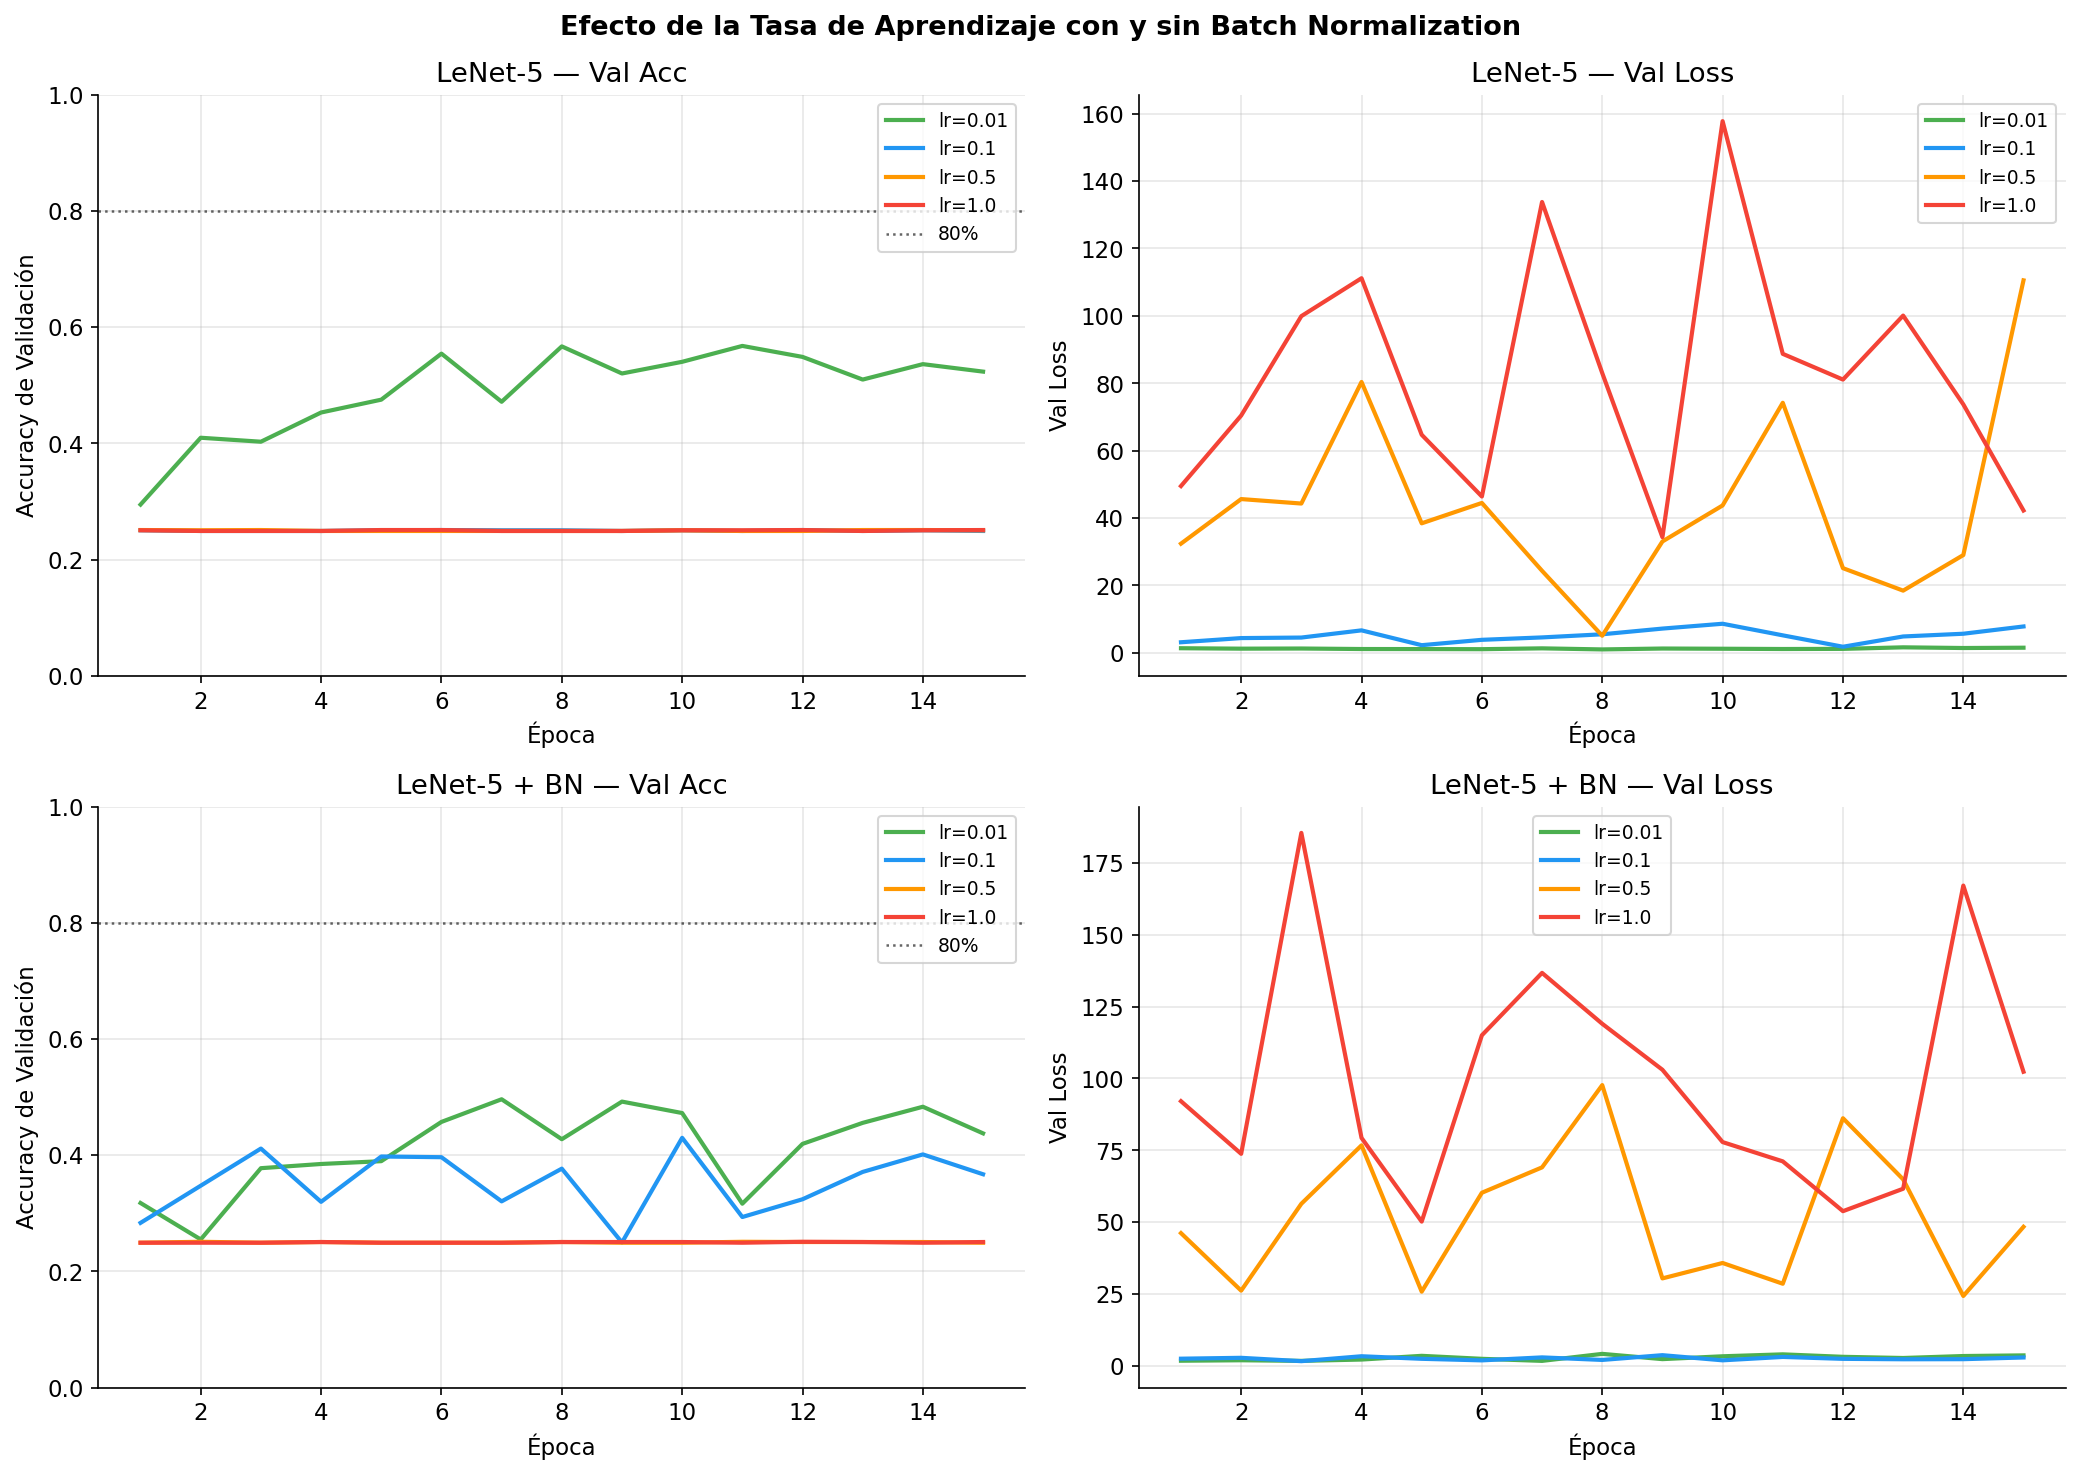
\includegraphics[width=0.92\textwidth]{results/lr_experiment.png}
\caption{Learning rate experiment for LeNet-5 with and without Batch Normalization.}
\label{fig:lr}
\end{figure}

\subsection{Feature maps}

Feature maps from the first convolutional layer were captured during training. In LeNet-5, the initial maps showed poorly structured patterns; as the epochs progressed, responses to edges, textures, and contrast regions appeared. The variant with Batch Normalization showed maps with greater contrast and specialization, although this did not translate into better test accuracy.

In the reduced VGG-11, the comparison was clearer: the version with Batch Normalization generated more stable and useful activations from early epochs, while the version without normalization maintained uninformative responses, consistent with its lack of convergence.

\begin{figure}[H]
\centering
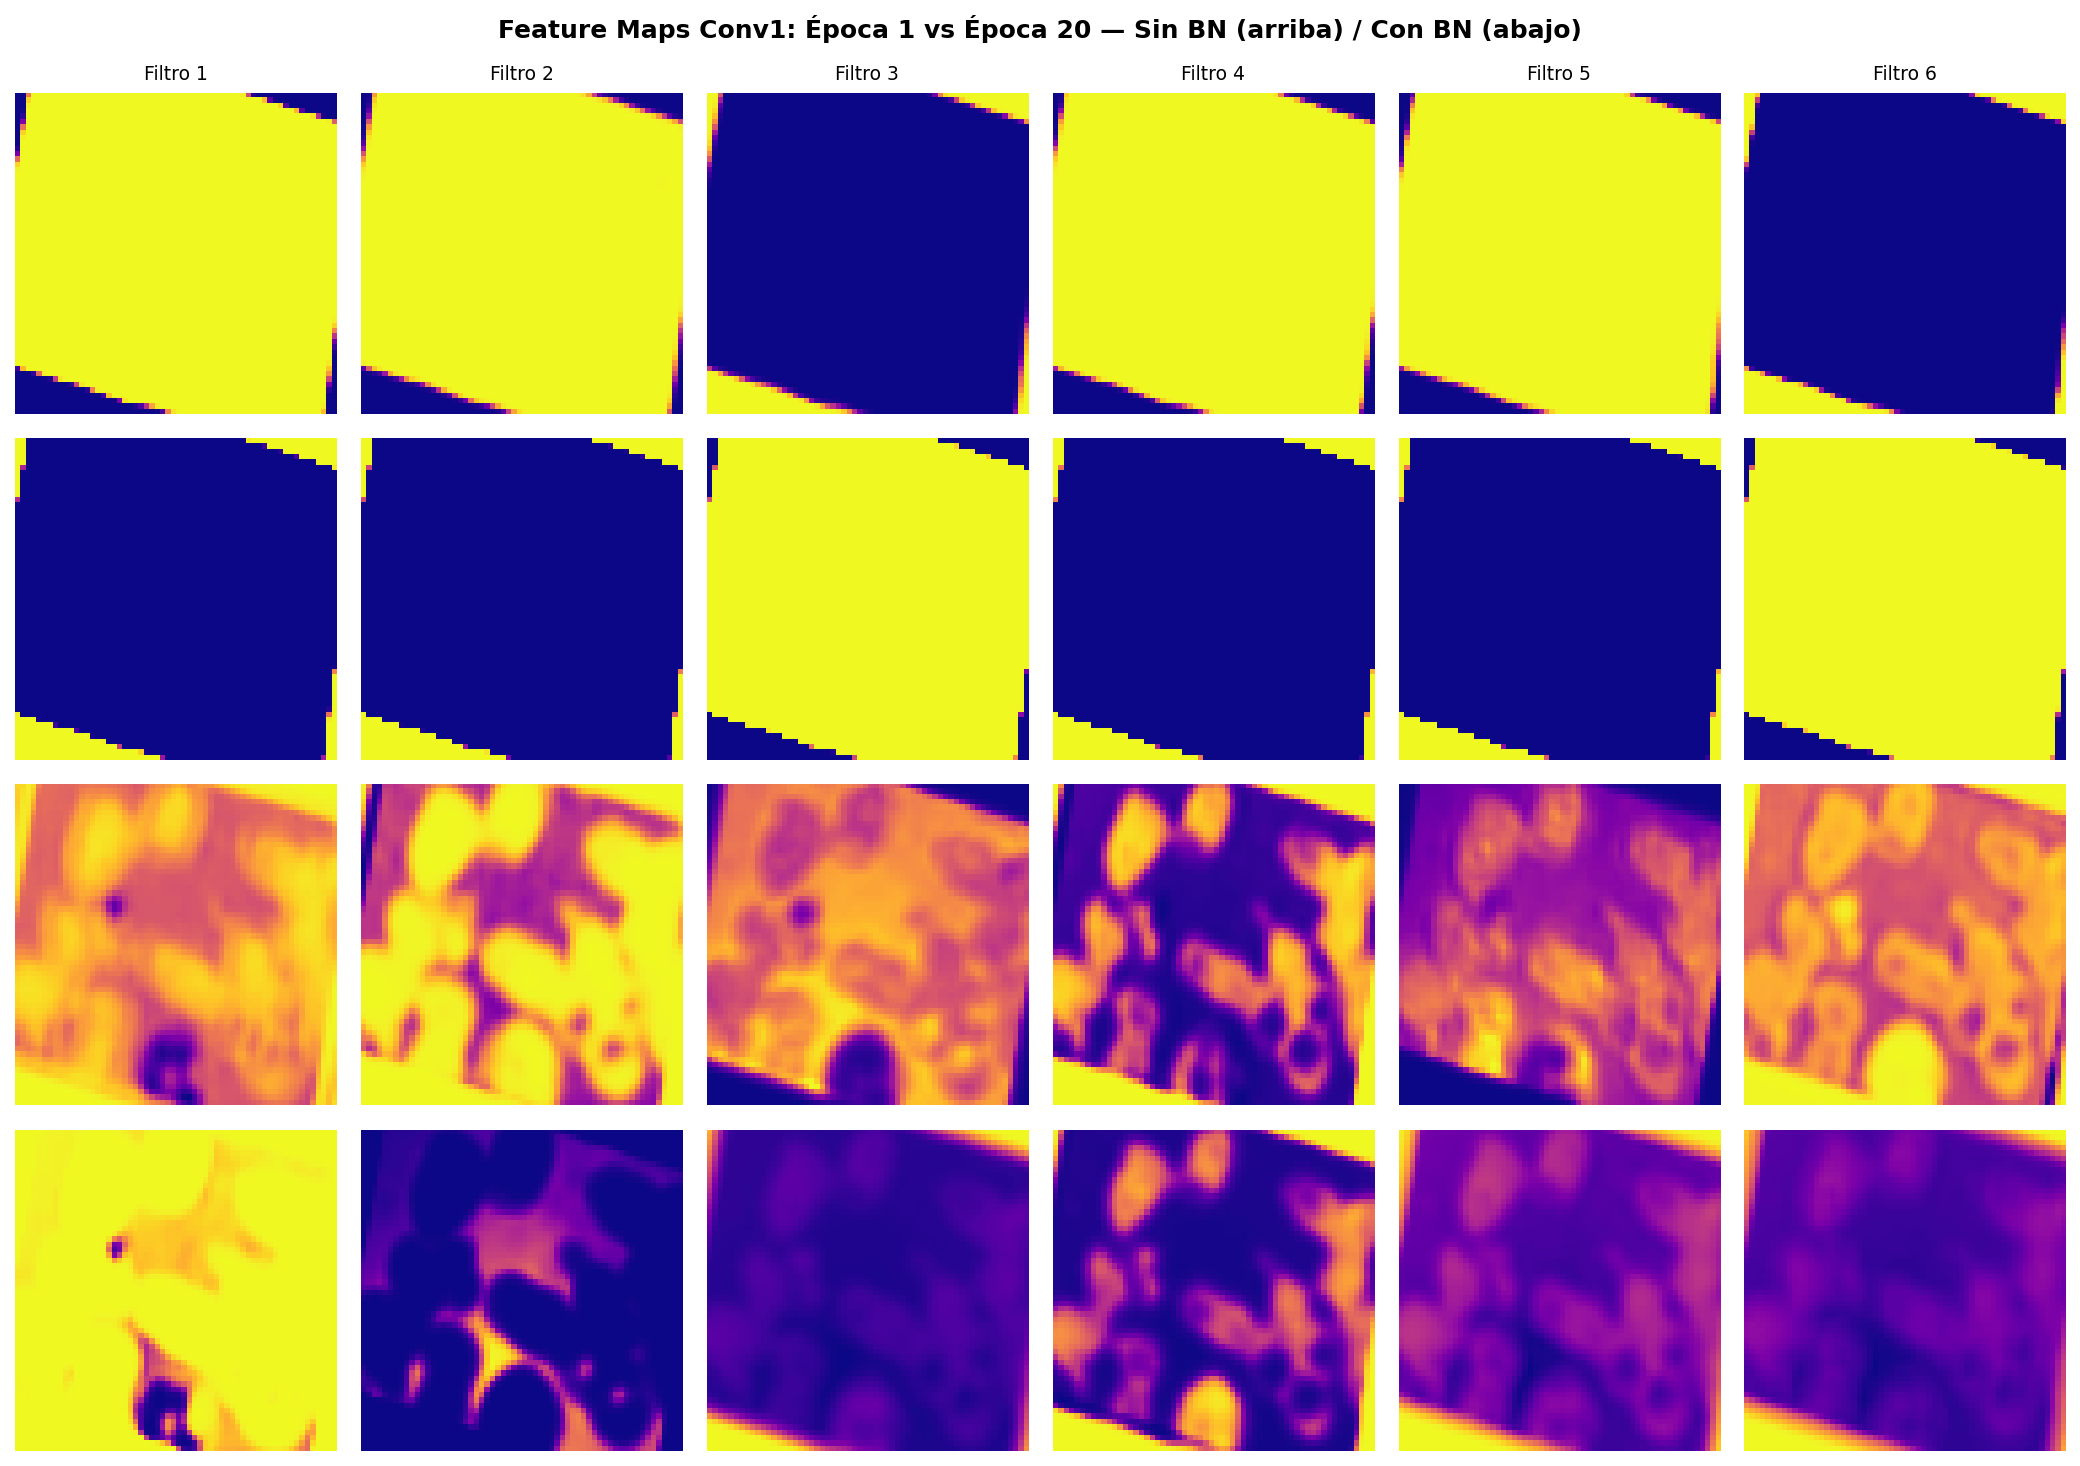
\includegraphics[width=0.92\textwidth]{results/fmaps_comparison.png}
\caption{Comparison of feature maps in LeNet-5, at the beginning and end of training.}
\label{fig:fmaps-lenet}
\end{figure}

\begin{figure}[H]
\centering
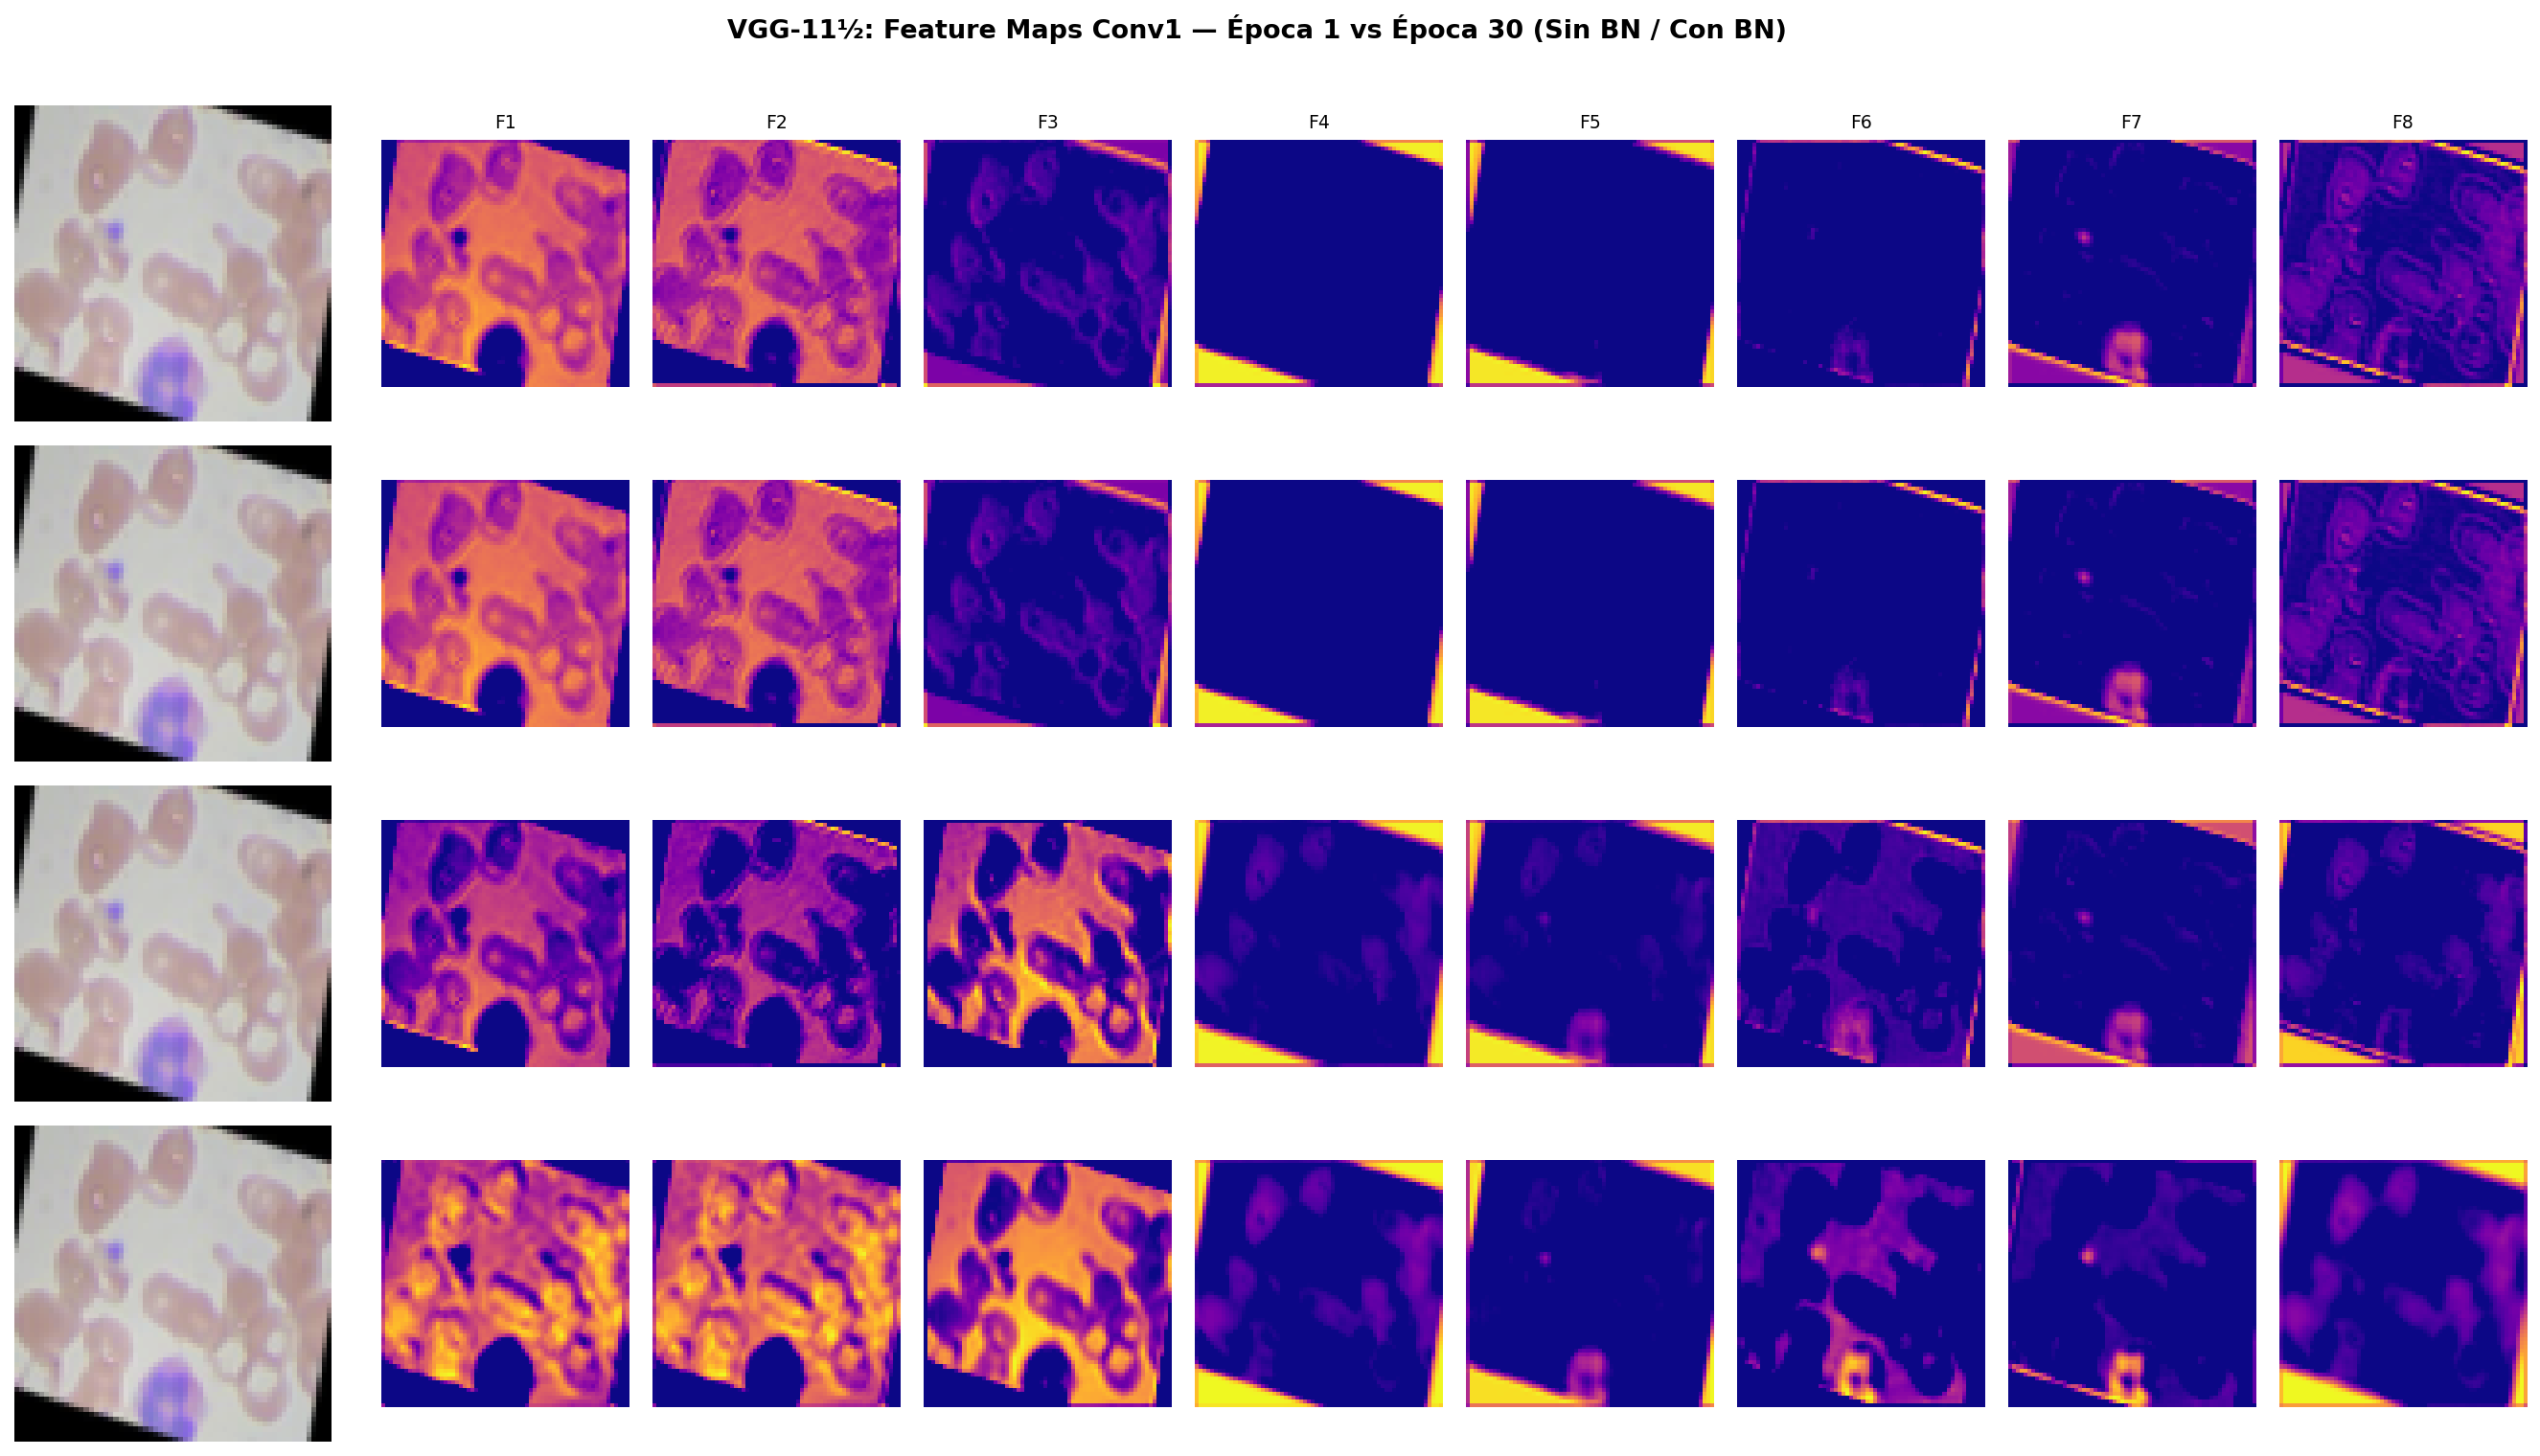
\includegraphics[width=0.92\textwidth]{results/fmaps_vgg11_half_training_comparison.png}
\caption{Comparison of feature maps in the reduced VGG-11 with and without Batch Normalization.}
\label{fig:fmaps-vgg}
\end{figure}

\subsection{Transfer learning}

Table~\ref{tab:transfer} summarizes the transfer learning results with ResNet18. Partial fine-tuning obtained the best result, with 86.45\% test accuracy. Full fine-tuning was very close, with 86.09\%, while feature extraction was considerably lower.

\begin{table}[H]
\centering
\caption{Transfer learning results with ResNet18.}
\label{tab:transfer}
\begin{tabular}{lrrrr}
\toprule
Strategy & TEST accuracy & Trainable params. & Total params. & Time \\
\midrule
Feature extraction & 45.96\% & 2052 & 11178564 & 7.75 min \\
Partial fine-tuning & 86.45\% & 10495492 & 11178564 & 7.61 min \\
Full fine-tuning & 86.09\% & 11178564 & 11178564 & 7.73 min \\
\bottomrule
\end{tabular}
\end{table}

The low performance of feature extraction indicates that training only the final layer is not enough to adapt ImageNet representations to the blood cell domain. Although early ImageNet filters capture general edges and textures, deeper layers encode visual concepts far from cellular morphology. Partial fine-tuning offers a better balance: it preserves generic early representations and adapts deeper layers to the specific domain. Full fine-tuning did not clearly outperform partial fine-tuning, suggesting that training all parameters may increase the risk of overfitting without providing a proportional gain.

\begin{figure}[H]
\centering
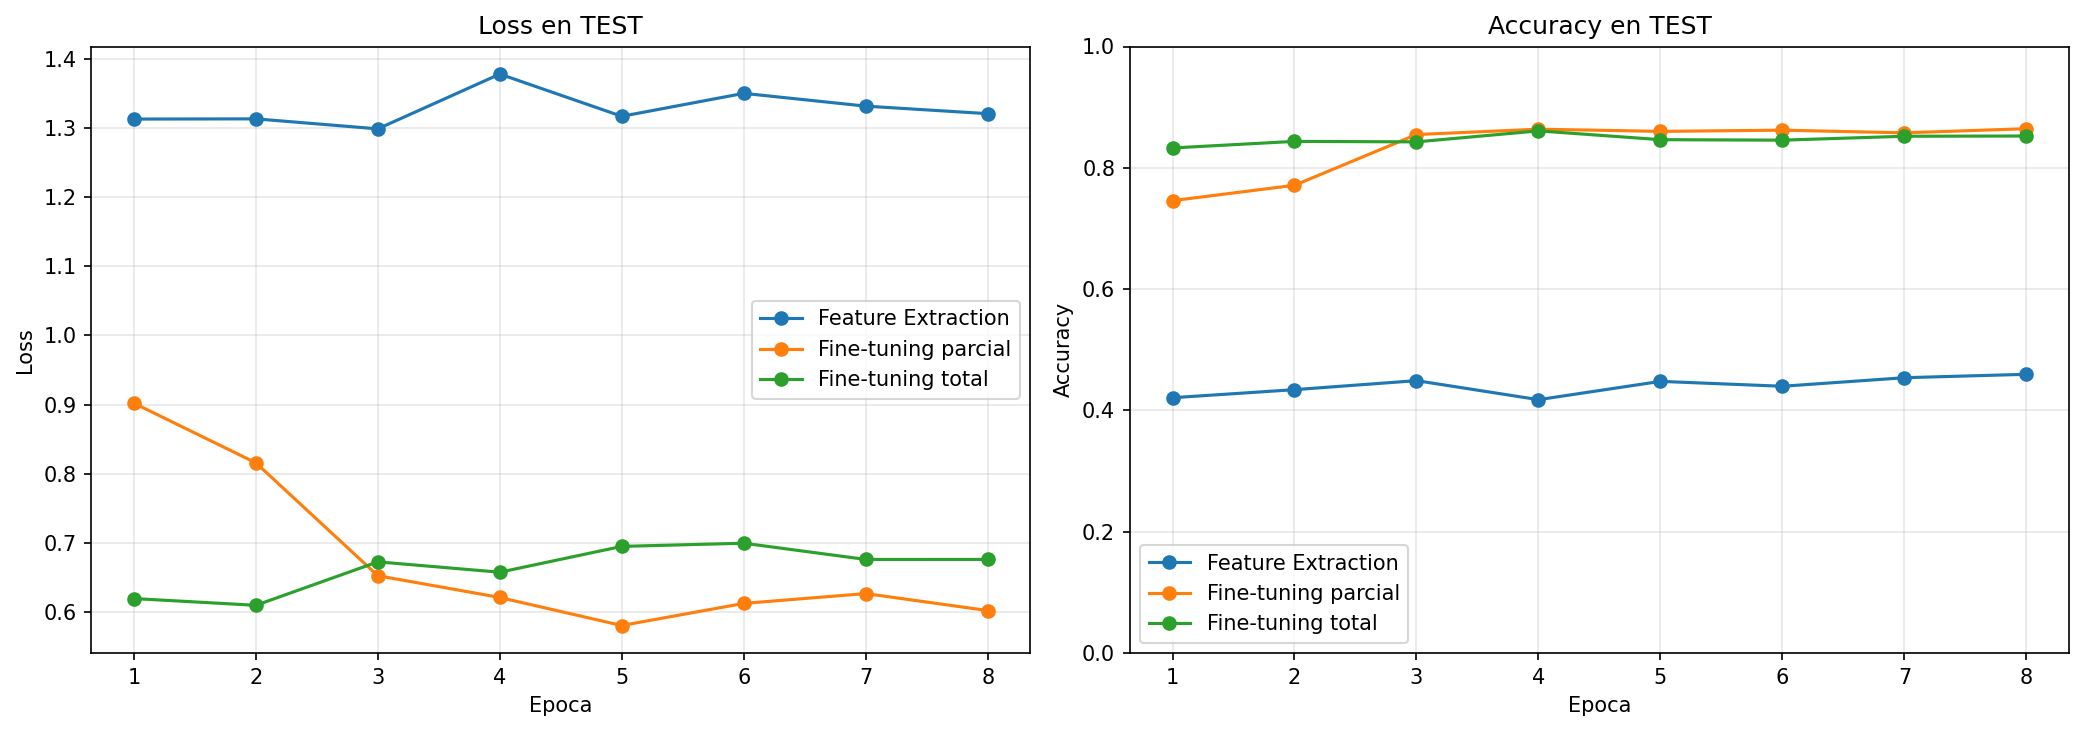
\includegraphics[width=0.92\textwidth]{results/transfer_learning_curves.png}
\caption{Training and test curves for the transfer strategies.}
\label{fig:transfer-curves}
\end{figure}

\begin{figure}[H]
\centering
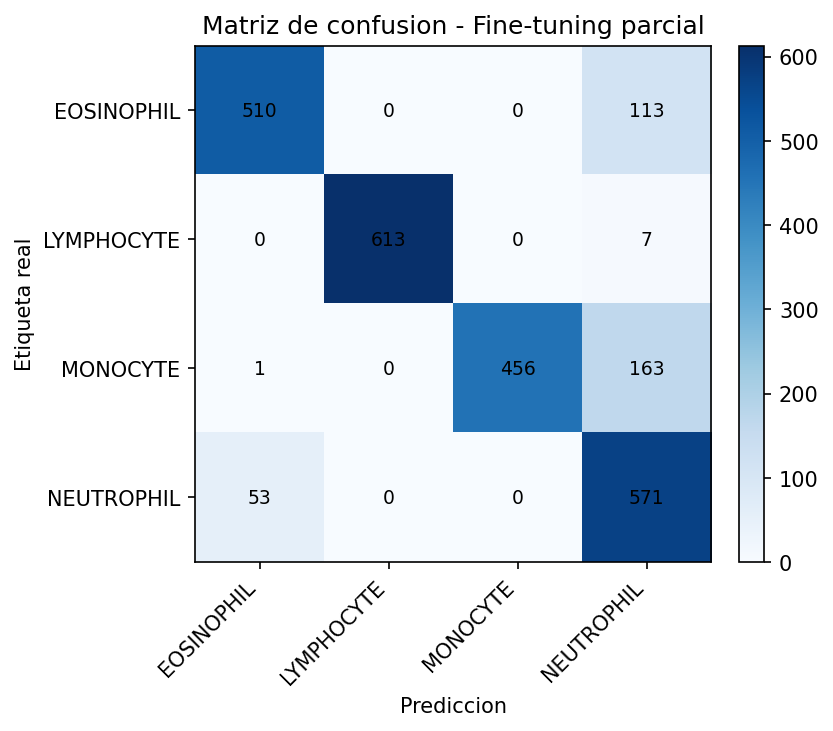
\includegraphics[width=0.82\textwidth]{results/best_transfer_confusion_matrix.png}
\caption{Confusion matrix of the best transferred model.}
\label{fig:confusion}
\end{figure}

\subsection{Global comparison}

The final comparison, presented in Table~\ref{tab:global}, shows that transfer learning was the most effective strategy. ResNet18 with partial fine-tuning outperformed the best model trained from scratch by approximately 5.23 percentage points.

\begin{table}[H]
\centering
\caption{Global comparison of the evaluated models.}
\label{tab:global}
\begin{tabular}{llc}
\toprule
Model & Source & Best TEST accuracy \\
\midrule
Partial fine-tuning & ResNet18 ImageNet & 86.45\% \\
Full fine-tuning & ResNet18 ImageNet & 86.09\% \\
Reduced VGG-11 + BN & From scratch & 81.22\% \\
LeNet-5 & From scratch & 58.22\% \\
Feature extraction & ResNet18 ImageNet & 45.96\% \\
LeNet-5 + BN & From scratch & 43.83\% \\
Reduced VGG-11 & From scratch & 25.09\% \\
\bottomrule
\end{tabular}
\end{table}

\begin{figure}[H]
\centering
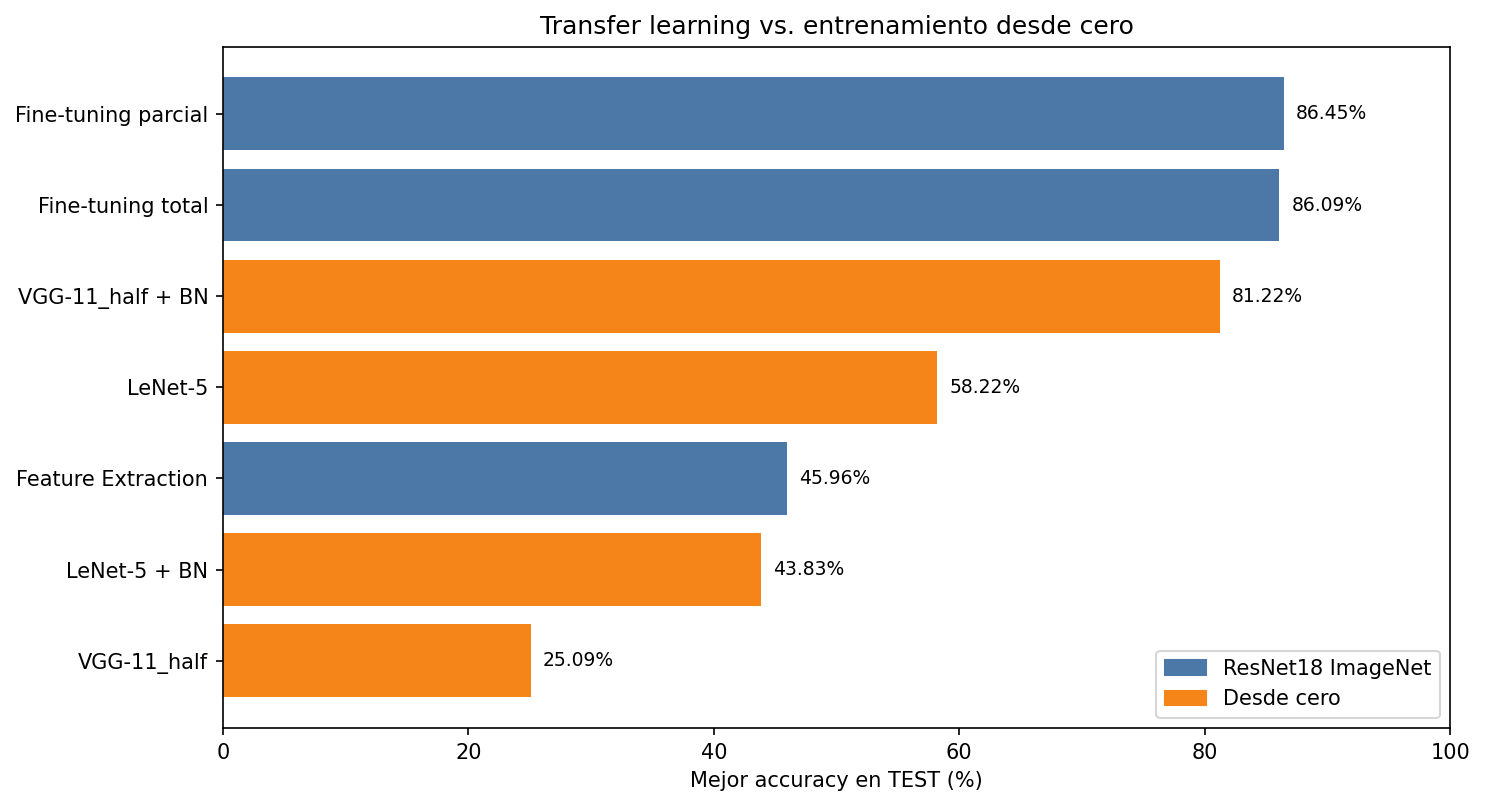
\includegraphics[width=0.9\textwidth]{results/transfer_vs_scratch_comparison.png}
\caption{Comparison between models trained from scratch and transfer strategies.}
\label{fig:global}
\end{figure}

\section{Critical analysis}

The results support three main conclusions. First, depth alone does not guarantee good performance: the reduced VGG-11 without Batch Normalization did not train effectively. Second, Batch Normalization can be essential for deep networks, but it does not replace a good regularization strategy or guarantee generalization in small models. Third, transfer learning was clearly superior when deeper layers were allowed to adapt to the cellular domain.

Nevertheless, there are important limitations. The first is the possible data leakage detected in the EDA: 48 source identifiers appear in more than one partition, and exact duplicates exist. If very similar images or images derived from the same origin appear in both training and testing, the reported accuracy may be optimistic. The second limitation is that \texttt{TEST} was repeatedly used as an evaluation set during development, so it also partially functioned as a model selection set. A more robust evaluation would require splitting \texttt{TRAIN} into training and validation, reserving \texttt{TEST} for a single final evaluation, and removing duplicates or grouping by source identifier before splitting.

Overfitting is also observed. LeNet-5 + BN reached high training accuracy but low test performance; partial fine-tuning reached more than 99\% in training from the first epochs, while testing stabilized around 86\%. Although this does not invalidate the result, it indicates that it would be advisable to report per-class metrics, confidence intervals, and external evaluation if the objective were applied use.

\section{Conclusions}

The best model in the project was ResNet18 with partial fine-tuning, with 86.45\% accuracy on TEST. This strategy represents the best observed compromise between domain adaptation, stability, and performance. Full fine-tuning obtained a very similar result, but without enough improvement to justify training all parameters as the first option. The best model trained from scratch was the reduced VGG-11 with Batch Normalization, with 81.22\%, confirming the importance of normalization in deep architectures.

As future work, it is recommended to rebuild the partitions by removing duplicates and grouping by source identifier, introduce an independent validation set, repeat training with several seeds, report precision, recall, and F1-score per class, and evaluate regularization techniques such as early stopping, more controlled augmentation, and progressive fine-tuning.

\begin{thebibliography}{9}

\bibitem{lecun1998gradient}
Y. LeCun, L. Bottou, Y. Bengio, and P. Haffner.
\textit{Gradient-based learning applied to document recognition}.
Proceedings of the IEEE, 86(11), 2278--2324, 1998.

\bibitem{simonyan2014very}
K. Simonyan and A. Zisserman.
\textit{Very Deep Convolutional Networks for Large-Scale Image Recognition}.
arXiv:1409.1556, 2014.

\bibitem{ioffe2015batch}
S. Ioffe and C. Szegedy.
\textit{Batch Normalization: Accelerating Deep Network Training by Reducing Internal Covariate Shift}.
Proceedings of the 32nd International Conference on Machine Learning, 37, 448--456, 2015.

\bibitem{santurkar2018does}
S. Santurkar, D. Tsipras, A. Ilyas, and A. Madry.
\textit{How Does Batch Normalization Help Optimization?}
Advances in Neural Information Processing Systems, 2018.

\bibitem{he2016deep}
K. He, X. Zhang, S. Ren, and J. Sun.
\textit{Deep Residual Learning for Image Recognition}.
Proceedings of the IEEE Conference on Computer Vision and Pattern Recognition, 770--778, 2016.

\bibitem{deng2009imagenet}
J. Deng, W. Dong, R. Socher, L.-J. Li, K. Li, and L. Fei-Fei.
\textit{ImageNet: A Large-Scale Hierarchical Image Database}.
IEEE Conference on Computer Vision and Pattern Recognition, 248--255, 2009.

\end{thebibliography}

\end{document}
